% TO DO:
% Are there any parameters that should be marked as Optional or Experimental?


% NOTES:
% Some of the parameter definitions in the appendix have R-specific flavor to them.  For example, c(100,100) is specific to R.
% Some of the parameters listed here are not available in R (and probably Python).  For example, _target_ratio_comm_to_comp
% Some references are in parenthesis and some are not.... need to standardize citations in text
% A few of the arguments are deprecated (according to Arno), but they still appear in the code, so I don't know if we should include them or not in our arg list.  Right now they appear as "(Deprecated)" below
% On the arglist, what does Optional indicate?  Many are not marked as optional... but are actually Optional.  Not sure (Optional) is being used properly.
% Many of the params in the arglist are shared with other algos, let's make sure those definitions are identical between booklets.
% Maybe move the Load Data section to the Use Case section (like GBM)


%\documentclass[a4paper, twoside]{article}
\setcounter{secnumdepth}{5}
\setcounter{tocdepth}{5}
\usepackage[english]{babel}
\usepackage{textcomp}
\usepackage{amsmath,amsthm,amsfonts,amssymb,epsfig}
\usepackage{array}
\usepackage{datetime}
\usepackage{lipsum}% http://ctan.org/pkg/lipsum
\usepackage[left=1.1in,top=1in,right=1.1in]{geometry}% http://ctan.org/pkg/geometry
\usepackage{listings}% http://ctan.org/pkg/listings
\usepackage{spverbatim}
\usepackage{hyperref}
\usepackage{microtype}
\hypersetup{colorlinks=true, urlcolor=black, linkcolor=black}
\usepackage{graphicx}
\graphicspath{ {images/} }
\usepackage{parskip}
\usepackage{titlesec} %used for diminishing heading sizes
\usepackage[square, sort, comma, numbers]{natbib} %%uses titles for cited references
\usepackage[fit]{truncate}
\usepackage{fancyhdr}
\pagestyle{fancy}
\fancyhead{}
\fancyhead[RO, RE]{\thepage}
\fancyhead[LO, LE]{\rightmark}
\renewcommand{\sectionmark}[1]{\markboth{}{\textsc{\thesection~#1}}}
\fancyfoot[C]{}%hide footer
\usepackage{xcolor} 
\usepackage[scaled=1]{couriers}

\xdefinecolor{gray}{rgb}{0.6,0.6,0.6} 
\documentclass[twoside]{article}
\usepackage[top=1in, left=0.5in, right=0.5in, bottom=0.5in,paperheight=8.5in,paperwidth=5.5in]{geometry}
\setcounter{secnumdepth}{5}
\setcounter{tocdepth}{5}
\usepackage[english]{babel}
\usepackage{textcomp}
\usepackage{amsmath,amsthm,amsfonts,amssymb,epsfig}
\usepackage{array}
\usepackage{datetime}
\usepackage{lipsum}% http://ctan.org/pkg/lipsum
\usepackage{listings}% http://ctan.org/pkg/listings
\usepackage{spverbatim}
\usepackage[hidelinks]{hyperref}
\Urlmuskip=0mu plus 1mu\relax %needed to make long URLs break nicely
\usepackage{microtype}
\hypersetup{colorlinks=false}
\usepackage{graphicx}
\graphicspath{ {images/} }
\usepackage{parskip}
\usepackage{titlesec} %used for diminishing heading sizes
\titleformat{\section}{\normalfont\bfseries}{\thesection}{1em}{}
\titlespacing*{\section}{0pt}{*2}{0pt}
\titlespacing*{\subsection}{0pt}{*2}{0pt}
\usepackage[square, sort, comma, numbers]{natbib} %%uses titles for cited references
\usepackage[fit]{truncate}
\usepackage{fancyhdr}
\pagestyle{fancy}
\renewcommand{\sectionmark}[1]{\markboth{#1}{}}
\fancyhead{}
\fancyhead[OR]{\leftmark \hspace{0.1cm}  $\vert$ \hspace{0.1cm}  \thepage}
\fancyhead[EL]{\thepage \hspace{0.1cm} $\vert$ \hspace{0.1cm} \leftmark}
\fancyfoot[C]{}%hide footer
\usepackage{xcolor} 
\usepackage[scaled=1]{couriers}
\usepackage{graphicx}
\xdefinecolor{gray}{rgb}{0.6,0.6,0.6} 
\usepackage{setspace}
\usepackage{adjustbox} 

  %settings for printed booklets - comment out by default, uncomment for print and comment out line above. don't save this change! "conf_top" should be default
\usepackage{bibentry}

\titleformat*{\section}{\LARGE\bfseries\sffamily}
\titleformat*{\subsection}{\Large\bfseries\sffamily}
\titleformat*{\subsubsection}{\large\bfseries\sffamily}
\titleformat*{\paragraph}{\large\bfseries\sffamily}
\titleformat*{\subparagraph}{\large\bfseries\sffamily}
\renewcommand{\familydefault}{\sfdefault} %sans-serif font



\begin{document}

%----------------------------------------------------------------------
% Definition for "lstlisting" blocks
%----------------------------------------------------------------------
% --- USAGE ---
%
% \begin{lstlisting}[style=R}
% ...
% \end{lstlisting}
%
% % \begin{lstlisting}[style=output}
% ...
% \end{lstlisting}
%----------------------------------------------------------------------

% By default, make listings all black so it's easy to spot the ones that aren't set to a style.
% This is just a debugging technique.
\lstset{backgroundcolor=\color{black}}

% Define scala language first
% ``define'' Scala
\lstdefinelanguage{scala}{
  morekeywords={abstract,case,catch,class,def,%
    do,else,extends,false,final,finally,%
    for,if,implicit,import,match,mixin,%
    new,null,object,override,package,%
    private,protected,requires,return,sealed,%
    super,this,throw,trait,true,try,%
    type,val,var,while,with,yield},
  otherkeywords={=>,<-,<\%,<:,>:,\#,@},
  sensitive=true,
  morecomment=[l]{//},
  morecomment=[n]{/*}{*/},
  morestring=[b]``,
  morestring=[b]',
  morestring=[b]''``
}

\lstdefinestyle{R}{
  language=R,
  frame=single,
  breaklines,
  basicstyle=\ttfamily,
  commentstyle=\textbf,% comment style
  keywordstyle=\ttfamily,
  numbers=left,% display line numbers on the left side 
  numberstyle=\scriptsize,% use small line numbers 
  numbersep=10pt,% space between line numbers and code
  backgroundcolor=\color{white}, 
  showstringspaces=false % don't show spaces as weird char.
}

\lstdefinestyle{python}{
  language=python,
  frame=single,
  breaklines,
  basicstyle=\ttfamily,
  commentstyle=\textsl,% comment style
  keywordstyle=\ttfamily,
  numbers=left,% display line numbers on the left side 
  numberstyle=\scriptsize,% use small line numbers 
  numbersep=10pt,% space between line numbers and code
  backgroundcolor=\color{white}, 
  showstringspaces=false %don't show spaces as weird char.
}

\lstdefinestyle{Scala}{
  language=scala,
  frame=single,
  breaklines,
  basicstyle=\ttfamily,
  commentstyle=\textsl,% comment style
  keywordstyle=\ttfamily,
  numbers=left,% display line numbers on the left side 
  numberstyle=\scriptsize,% use small line numbers 
  numbersep=10pt,% space between line numbers and code
  backgroundcolor=\color{white}, 
  showstringspaces=false % don't show spaces as weird char.
}

\lstdefinestyle{Bash}{
  language=bash,
  frame=single,
  breaklines,
  basicstyle=\ttfamily,
  commentstyle=\textsl,% comment style
  keywordstyle=\ttfamily,
  numbers=left,% display line numbers on the left side 
  numberstyle=\scriptsize,% use small line numbers 
  numbersep=10pt,% space between line numbers and code
  backgroundcolor=\color{white}, 
  showstringspaces=false % don't show spaces as weird char.
}


\definecolor{mygray}{rgb}{0.92,0.92,0.92}

\lstdefinestyle{output}{
  frame=single,
  breaklines,
  basicstyle=\ttfamily,
  numbers=left,% display line numbers on the left side 
  numberstyle=\scriptsize,% use small line numbers 
  numbersep=10pt,% space between line numbers and code
  backgroundcolor=\color{mygray}, 
  showstringspaces=false %don't show spaces as weird char.
}

\newcommand{\waterExampleInR} {
\textbf{Example in R} \\
}

\newcommand{\waterExampleInPython} {
\textbf{Example in Python} \\
}
 %see note for `conf_top_print.tex` above
%% TO DO: Find better templates for R and Python



%----------------------------------------------------------------------
% Definition for "lstlisting" blocks
%----------------------------------------------------------------------
% --- USAGE ---
%
% \begin{lstlisting}[style=R}
% ...
% \end{lstlisting}
%
% % \begin{lstlisting}[style=output}
% ...
% \end{lstlisting}
%----------------------------------------------------------------------

% By default, make listings all black so it's easy to spot the ones that aren't set to a style.
% This is just a debugging technique.
%\lstset{backgroundcolor=\color{black}}

% http://latexcolor.com/
\definecolor{deepblue}{rgb}{0,0,0.5}
\definecolor{deepred}{rgb}{0.6,0,0}
\definecolor{deepgreen}{rgb}{0,0.5,0}
%\definecolor{tan}{rgb}{0.98, 0.92, 0.84}  %antiquewhite
%\definecolor{r_bkgd}{rgb}{1.0, 0.92, 0.8}  %blacnedalmond
\definecolor{py_bkgd}{rgb}{0.94, 0.97, 1.0}  %aliceblue
\definecolor{ashgrey}{rgb}{0.7, 0.75, 0.71}
\definecolor{battleshipgrey}{rgb}{0.52, 0.52, 0.51}
%\definecolor{r_bkgd}{rgb}{0.97, 0.91, 0.81}  %champagne
\definecolor{r_bkgd}{rgb}{0.98, 0.92, 0.84}  %moccasin

\definecolor{Code}{rgb}{0,0,0}
\definecolor{Decorators}{rgb}{0.5,0.5,0.5}
\definecolor{Numbers}{rgb}{0.5,0,0}
\definecolor{MatchingBrackets}{rgb}{0.25,0.5,0.5}
\definecolor{Keywords}{rgb}{0,0,1}
\definecolor{self}{rgb}{0,0,0}
\definecolor{Strings}{rgb}{0,0.63,0}
\definecolor{Comments}{rgb}{0,0.63,1}
\definecolor{Backquotes}{rgb}{0,0,0}
\definecolor{Classname}{rgb}{0,0,0}
\definecolor{FunctionName}{rgb}{0,0,0}
\definecolor{Operators}{rgb}{0,0,0}
\definecolor{Background}{rgb}{0.98,0.98,0.98}

% KEYWORDS
% http://tex.stackexchange.com/questions/186092/how-can-i-delete-non-letter-keywords-such-as
\lstdefinestyle{Scala}{
  language={Scala},
  frame=single,
  breaklines,
  basicstyle=\ttfamily,
  commentstyle=\itshape\color{battleshipgrey},% comment style
  %commentstyle=\textsl,% comment style
  %keywordstyle=\ttfamily\color{deepblue},
  %keywordstyle=\color{WildStrawberry},
  numbers=left,% display line numbers on the left side
  numberstyle=\scriptsize,% use small line numbers
  numbersep=10pt,% space between line numbers and code
  backgroundcolor=\color{white},
  showstringspaces=false,
  stringstyle=\color{deepgreen},
  backgroundcolor=\color{py_bkgd},
  % keywords
  morekeywords={abstract,case,catch,class,def,%
    do,else,extends,false,final,finally,%
    for,if,implicit,import,match,mixin,%
    new,null,object,override,package,%
    private,protected,requires,return,sealed,%
    super,this,throw,trait,true,try,%
    type,val,var,while,with,yield},
  otherkeywords={=>,<-,<\%,<:,>:,\#,@},
  sensitive=true,
  morecomment=[l]{//},
  morecomment=[n]{/*}{*/},
  morestring=[b]``,
  morestring=[b]',
  morestring=[b]''``,
  keywordstyle={\color{Keywords}\bfseries},
}

\lstdefinestyle{R}{
  language={R},
  frame=single,
  breaklines,
  basicstyle=\ttfamily,
  %commentstyle=\textsl\color{Comments},% comment style
  commentstyle=\itshape\color{battleshipgrey},% comment style
  keywordstyle=\ttfamily\color{deepblue},
  numbers=left,% display line numbers on the left side 
  numberstyle=\scriptsize,% use small line numbers 
  numbersep=10pt,% space between line numbers and code
  backgroundcolor=\color{r_bkgd},
  showstringspaces=false,
  stringstyle=\color{deepgreen},
  %morekeywords={TRUE, FALSE, for, if},
  keywordstyle={\color{Keywords}\bfseries},
  keywords={TRUE, FALSE},
  deletekeywords={grid, frame, variable, model, vi, predict, file},
  otherkeywords={!,!=,~,$,*,\&,\%/\%,\%*\%,\%\%,<-,<<-},
  %morekeywords={TRUE, FALSE, list, c}
}



\lstdefinestyle{python}{
  language={Python},
  frame=single,
  breaklines,
  basicstyle=\ttfamily,
  commentstyle=\itshape\color{battleshipgrey},% comment style
  %commentstyle=\textsl,% comment style
  %keywordstyle=\ttfamily\color{deepblue},
  %keywordstyle=\color{WildStrawberry},
  numbers=left,% display line numbers on the left side 
  numberstyle=\scriptsize,% use small line numbers 
  numbersep=10pt,% space between line numbers and code
  backgroundcolor=\color{white},
  showstringspaces=false,
  stringstyle=\color{deepgreen},
  backgroundcolor=\color{py_bkgd},
  % keywords
morekeywords={import,from,class,def,for,while,if,is,in,elif,else,not,and,or,print,break,continue,return,True,False,None,access,as,,del,except,exec,finally,global,import,lambda,pass,print,raise,try,assert},
 keywordstyle={\color{Keywords}\bfseries},
}

\lstdefinestyle{Bash}{
  language=bash,
  frame=single,
  breaklines,
  basicstyle=\ttfamily,
  commentstyle=\textsl,% comment style
  keywordstyle=\ttfamily,
  numbers=left,% display line numbers on the left side
  numberstyle=\scriptsize,% use small line numbers
  numbersep=10pt,% space between line numbers and code
  backgroundcolor=\color{white},
  showstringspaces=false % don't show spaces as weird char.
}

\definecolor{mygray}{rgb}{0.92,0.92,0.92}

\lstdefinestyle{output}{
  frame=single,
  breaklines,
  basicstyle=\ttfamily,
  numbers=left,% display line numbers on the left side 
  numberstyle=\scriptsize,% use small line numbers 
  numbersep=10pt,% space between line numbers and code
  backgroundcolor=\color{mygray},
  showstringspaces=false 
}

\newcommand{\waterExampleInR} {
\textbf{Example in R} \\
}

\newcommand{\waterExampleInPython} {
\textbf{Example in Python} \\
}
  %Use this for online version


\thispagestyle{empty} %removes page number
\newgeometry{bmargin=0cm, hmargin=0cm}


\begin{center}
\textsc{\Large\bf{Deep Learning with H2O}}
\bigskip

\line(1,0){250}  %inserts  horizontal line



\bigskip

\textsc{\small{Arno Candel \hspace{10pt} Viraj Parmar \hspace{10pt} Erin LeDell  \hspace{10pt} Anisha Arora}}

\textsc{\small{Edited by: Jessica Lanford}}

\line(1,0){250}  %inserts  horizontal line

{\url{http://h2o.ai/resources/}}

\normalsize
\bigskip
\monthname \hspace{1pt}  \the\year: Fourth Edition 

\bigskip
\end{center}

% commenting out lines image due to print issues, but leaving in for later
%\null\vfill
%\begin{figure}[!b]
%\noindent\makebox[\textwidth]{%
%\centerline{
\includegraphics[width=\paperwidth]{waves.png}}}
%\end{figure}


\newpage
\restoregeometry

\null\vfill %move next text block to lower left of new page

\thispagestyle{empty}%remove pg#
{\raggedright\vfill\ 

Deep Learning with H2O\\

by Arno Candel, Erin LeDell,\\
Viraj Parmar,  \&\ Anisha Arora  \\
Edited by: Jessica Lanford

\bigskip
  Published by H2O.ai, Inc. \\
2307 Leghorn St. \\
Mountain View, CA 94043\\
\bigskip
\textcopyright 2015 H2O.ai, Inc. All Rights Reserved. 
\bigskip

\monthname \hspace{1pt}  \the\year: Fourth Edition
\bigskip

Photos by \textcopyright H2O.ai, Inc. 
\bigskip

All copyrights belong to their respective owners.\\
While every precaution has been taken in the\\
preparation of this book, the publisher and\\
authors assume no responsibility for errors or\\
omissions, or for damages resulting from the\\
use of the information contained herein.\\
\bigskip
Printed in the United States of America. 
}

\newpage
\thispagestyle{empty}%remove pg#
\tableofcontents
\thispagestyle{empty}%remove pg#

%----------------------------------------------------------------------
%----------------------------------------------------------------------

\newpage

\section{Introduction}
This document introduces the reader to Deep Learning with H2O.  Examples are written in R and Python.
Topics include: 
\begin{itemize}
\item installation of H2O
\item basic Deep Learning concepts
\item building deep neural nets in H2O
\item how to interpret model output
\item how to make predictions
\end{itemize}
as well as various implementation details.

\section{What is H2O?}
\Urlmuskip=0mu plus 1mu\relax %needed to make long URLs break nicely


H2O is fast, scalable, open-source machine learning and deep learning for smarter applications. With H2O, enterprises like PayPal, Nielsen Catalina, Cisco, and others can use all their data without sampling to get accurate predictions faster. Advanced algorithms such as deep learning, boosting, and bagging ensembles are built-in to help application designers create smarter applications through elegant APIs. Some of our initial customers have built powerful domain-specific predictive engines for recommendations, customer churn, propensity to buy, dynamic pricing, and fraud detection for the insurance, healthcare, telecommunications, ad tech, retail, and payment systems industries.

Using in-memory compression, H2O handles billions of data rows in-memory, even with a small cluster. To make it easier for non-engineers to create complete analytic workflows, H2O's platform includes interfaces for R, Python, Scala, Java, JSON, and CoffeeScript/JavaScript, as well as a built-in  web interface, Flow. H2O was built alongside (and on top of) Hadoop and Spark Clusters and typically deploys within minutes.

H2O includes many common machine learning algorithms, such as generalized linear modeling (linear regression, logistic regression, etc.), Na\"{i}ve Bayes, principal components analysis, time series, k-means clustering, and others. H2O also implements best-in-class algorithms at scale, such as distributed random forest, gradient boosting and deep learning. Customers can build thousands of models and compare the results to get the best predictions.

H2O is nurturing a grassroots movement of physicists, mathematicians, and computer scientists to herald the new wave of discovery with data science by collaborating closely with academic researchers and Industrial data scientists. Stanford university giants Stephen Boyd, Trevor Hastie, Rob Tibshirani advise the H2O team on building scalable machine learning algorithms. With hundreds of meetups over the past three years, H2O has become a word-of-mouth phenomenon, growing amongst the data community by a hundred-fold, and is now used by 30,000+ users and is deployed using R, Python, Hadoop, and Spark in 2000+ corporations.

\textbf{Try it out}

\begin{itemize}
\item  Download H2O directly at \mbox{\url{http://h2o.ai/download}}.
\item Install H2O's R package from CRAN at {\url{https://cran.r-project.org/web/packages/h2o/}}. 
\item Install the Python package from PyPI at {\url{https://pypi.python.org/pypi/h2o/}}.

\end{itemize}



\textbf{Join the community}
\begin{itemize}
\item  To learn about our meetups, training sessions, hackathons, and product updates, visit {\url{http://h2o.ai}}. 
\item Visit the open source community forum at {\url{https://groups.google.com/d/forum/h2ostream}}.
\item Join the chat at {\url{https://gitter.im/h2oai/h2o-3}}.
\end{itemize}





\input{generated_buildinfo.tex}
\section{Installation} 
\Urlmuskip=0mu plus 1mu\relax %needed to make long URLs break nicely


The easiest way to directly install H2O is  via an R or Python package.

({\bf{Note}}: The examples in this document were created with H2O version \waterVersion.)

\subsection{Installation in R}

To load a recent H2O package from CRAN, run:

\begin{lstlisting}[style=R]
install.packages("h2o")
\end{lstlisting}

{\bf{Note}}: The version of H2O in CRAN is often one release behind the current version.

For the latest recommended version, download the
latest stable H2O-3 build from the H2O download page:

\begin{enumerate}
\item Go to {\url{http://h2o.ai/download}}.
\item Choose the latest stable H2O-3 build.
\item Click the ``Install in R'' tab.
\item Copy and paste the commands into your R session.
\end{enumerate}

\bigskip
After H2O is installed on your system, verify the installation:

\begin{lstlisting}[style=R]
library(h2o)

#Start H2O on your local machine using all available cores.
#By default, CRAN policies limit use to only 2 cores.
h2o.init(nthreads = -1)

#Get help
?h2o.glm
?h2o.gbm

#Show a demo
demo(h2o.glm)
demo(h2o.gbm)
\end{lstlisting}

\subsection{Installation in Python}

To load a recent H2O package from PyPI, run:

\begin{lstlisting}[style=python]
pip install h2o
\end{lstlisting}

To download the
latest stable H2O-3 build from the H2O download page:

\begin{enumerate}
\item Go to {\url{http://h2o.ai/download}}.
\item Choose the latest stable H2O-3 build.
\item Click the ``Install in Python'' tab.
\item Copy and paste the commands into your Python session.
\end{enumerate}

\bigskip
After H2O is installed, verify the installation:

\begin{lstlisting}[style=python]
import h2o

# Start H2O on your local machine
h2o.init()

# Get help
help(h2o.glm)
help(h2o.gbm)

# Show a demo
h2o.demo("glm")
h2o.demo("gbm")

\end{lstlisting}

\subsection{Pointing to a Different H2O Cluster}

The instructions in the previous sections create a one-node H2O cluster on your local machine. 

To connect to an established H2O cluster (in a multi-node Hadoop environment, for example) specify the IP address and port number for the established cluster using the \texttt{ip} and \texttt{port} parameters in the \texttt{h2o.init()} command.  The syntax for this function is identical for R and Python:
\medskip  

\begin{lstlisting}[style=R]
h2o.init(ip = "123.45.67.89", port = 54321)
\end{lstlisting}

%if it's the same, only one is needed



\subsection{Example Code}

R and Python code for the examples in this document can be found here:

\url{https://github.com/h2oai/h2o-3/tree/master/h2o-docs/src/booklets/v2_2015/source/DeepLearning_Vignette_code_examples}

The document source itself can be found here:

\url{https://github.com/h2oai/h2o-3/blob/master/h2o-docs/src/booklets/v2_2015/source/DeepLearning_Vignette.tex}
\newpage
\subsection{Citation}

To cite this booklet, use the following: 

Candel, A., Parmar, V., LeDell, E.,  and Arora, A. (Nov. 2015). {\textit{Deep Learning with H2O}}. {\url{http://h2o.ai/resources}}. 

\section{Deep Learning Overview}
Unlike the neural networks of the past, modern Deep Learning  provides training stability, generalization, and scalability with big data. Since it performs quite well in a number of diverse problems, Deep Learning is quickly becoming the algorithm of choice for the highest predictive accuracy. 

The first section is a brief overview of deep neural networks for supervised learning tasks. There are several theoretical frameworks for Deep Learning, but this document focuses primarily on the feedforward architecture used by H2O. 

The basic unit in the model (shown in the image below) is the neuron, a biologically inspired model of the human neuron. In humans, the varying strengths of the neurons' output signals travel along the synaptic junctions and are then aggregated  as input for a connected neuron's activation. 

In the model, the weighted combination $\alpha = \sum_{i=1}^{n} w_i x_i + b$ of input signals is aggregated, and then an output signal $f(\alpha)$ transmitted by the connected neuron. The function $f$ represents the nonlinear activation function used throughout the network and the bias $b$ represents the neuron's activation threshold.

\begin{figure}[h]
\centering
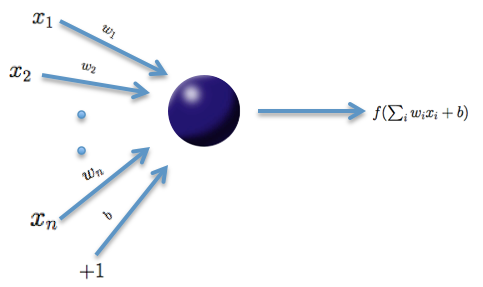
\includegraphics[scale=0.7]{neuron.png}
\end{figure}

Multi-layer, feedforward neural networks consist of many layers of interconnected neuron units (as shown in the following image), starting with an input layer to match the feature space, followed by multiple layers of nonlinearity, and ending with a linear regression or classification layer to match the output space. The inputs and outputs of the model's units follow the basic logic of the single neuron described above. 

\begin{figure}[ht]
\centering
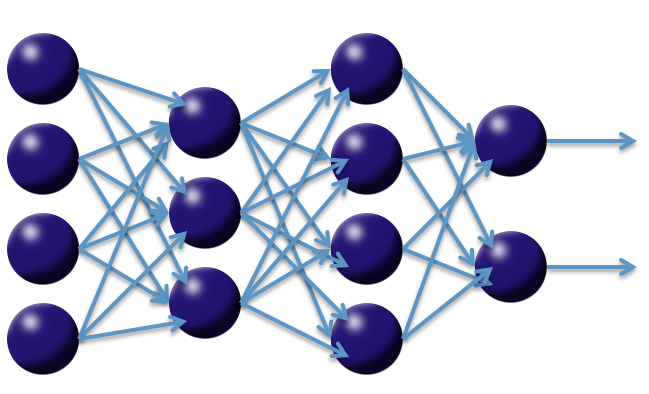
\includegraphics[scale=0.5]{net.png}
\end{figure}

Bias units are included in each non-output layer of the network. The weights linking neurons and biases with other neurons fully determine the output of the entire network. Learning occurs when these weights are adapted to minimize the error on the labeled training data. More specifically, for each training example $j$, the objective is to minimize a loss function, 
\begin{center}
$L(W,B$ $|$ $j)$.
\end{center}
Here, $W$ is the collection $\left\{W_i\right\}_{1:N-1}$, where $W_i$ denotes the weight matrix connecting layers $i$ and $i+1$ for a network of $N$ layers. Similarly $B$ is the collection $\left\{b_i\right\}_{1:N-1}$, where $b_i$ denotes the column vector of biases for layer $i+1$.

This basic framework of multi-layer neural networks can be used to accomplish Deep Learning tasks. Deep Learning architectures are models of hierarchical feature extraction, typically involving multiple levels of nonlinearity. Deep Learning models are able to learn useful representations of raw data and have exhibited high performance on complex data such as images, speech, and text \href{http://www.iro.umontreal.ca/~lisa/pointeurs/TR1312.pdf}{(Bengio, 2009)}. 

\section{H2O's Deep Learning Architecture} 

H2O follows the model of multi-layer, feedforward neural networks for predictive modeling. This section provides a more detailed description of H2O's Deep Learning features, parameter configurations, and computational implementation.

\newpage
\subsection{Summary of Features} 

H2O's Deep Learning functionalities include: 

\begin{itemize}

\item supervised training protocol for regression and classification tasks

\item fast and memory-efficient Java implementations based on columnar compression and fine-grain MapReduce

\item multi-threaded and distributed parallel computation that can be run on a single or a multi-node cluster

\item automatic, per-neuron, adaptive learning rate for fast convergence

\item optional specification of learning rate, annealing, and momentum options

\item regularization options such as L1, L2, dropout, \textsc{Hogwild!}, and model averaging to prevent model overfitting

\item elegant and intuitive web interface (Flow)

\item fully scriptable R API from H2O's CRAN package

\item fully scriptable Python API

\item grid search for hyperparameter optimization and model selection

\item automatic early stopping based on convergence of user-specified metrics to user-specified tolerance

\item model checkpointing for reduced run times and model tuning

\item automatic pre- and post-processing for categorical and numerical data

\item automatic imputation of missing values

\item automatic tuning of communication vs computation for best performance  %assuming this is a reference to the force_load_balance param?

\item model export in plain Java code for deployment in production environments

\item additional expert parameters for model tuning

\item deep autoencoders for unsupervised feature learning and anomaly detection 

\end{itemize}

\newpage
\subsection{Training Protocol} 
The training protocol described below follows many of the ideas and advances discussed in recent Deep Learning literature.

\subsubsection{Initialization}
\label{sssec:Initialization}

Various Deep Learning architectures employ a combination of unsupervised pre-training followed by supervised training, but H2O uses a purely supervised training protocol. The default initialization scheme is the uniform adaptive option, which is an optimized initialization based on the size of the network. Deep Learning can also be started using a random initialization drawn from either a uniform or normal distribution, optionally specifying a scaling parameter. \nowidow[6]


\subsubsection{Activation and Loss Functions} \label{sssec:ActivationLoss}
The choices for the nonlinear activation function $f$ described in the introduction are summarized in Table 1 below. $x_i$ and $w_i$ represent the firing neuron's input values and their weights, respectively; $\alpha$ denotes the weighted combination $\alpha = \sum_i w_i x_i+b$.

\begin{table}[ht] 
\caption{Activation Functions }
\smallskip
% title of Table 
\centering % used for centering table 
\begin{tabular}{c c c} % centered columns (4 columns) 
\hline\hline %inserts double horizontal lines 
Function & Formula & Range \\ [0.5ex] % inserts table 
%heading 
\hline % inserts single horizontal line 
Tanh & $f(\alpha) = \frac{e^{\alpha} - e ^{-\alpha}}{e^\alpha + e ^{-\alpha}}$ & $f(\cdot) \in [-1,1]$ \\ % inserting body of the table 
Rectified Linear & $f(\alpha) = \max(0,\alpha)$ & $f(\cdot) \in \mathbb{R}_+$ \\
Maxout & $f(\alpha_1,\alpha_2) = \max(\alpha_1,\alpha_2) $ & $f(\cdot) \in \mathbb{R}$\\  % [1ex] adds vertical space
\hline %inserts single line 
\end{tabular} 
\label{table:ActivationFunctions} % is used to refer this table in the text 
\end{table}

The $\tanh$ function is a rescaled and shifted logistic function; its symmetry around 0 allows the training algorithm to converge faster. The rectified linear activation function has demonstrated high performance on image recognition tasks and is a more biologically accurate model of neuron activations (\href{http://yann.lecun.com/exdb/publis/pdf/lecun-98b.pdf}{LeCun et al, 1998}). 

Maxout is a generalization of the \texttt{Rectifiied Linear} activation, where each neuron picks the largest output of $k$ separate channels, where each channel has its own weights and bias values. The current implementation supports only $k=2$. Maxout activation works particularly well with dropout (\href{http://arxiv.org/pdf/1302.4389.pdf}{Goodfellow et al, 2013}). For more information, refer to {\textbf{\nameref{ssec:Regularization}}}.

The Rectifier is the special case of Maxout where the output of one channel is always 0.
It is difficult to determine a ``best" activation function to use; each may outperform the others in separate scenarios, but grid search models can help to compare activation functions and other parameters.  For more information, refer to {\textbf{\nameref{ssec:GridSearch}}}. The default activation function is the Rectifier. Each of these activation functions can be operated with dropout regularization. For more information, refer to {\textbf{\nameref{ssec:Regularization}}}.

Specify the one of the following distribution functions for the response variable using the \texttt{distribution} argument: 

\begin{frame}%no line table for list of 6+ items

\begin{tabular}{p{4cm}p{4cm}p{4cm}}

\begin{itemize}
     \item AUTO
     \item Bernoulli
     \item Multinomial
  \end{itemize} &

\begin{itemize}
  \item Poisson
  \item Gamma
  \item Tweedie
\end{itemize} &

\begin{itemize}
  \item Laplace
  \item Huber
  \item Gaussian
\end{itemize}\\

\end{tabular}

\end{frame}

Each distribution has a primary association with a particular loss function, but some distributions allow users to specify a non-default loss function from the group of loss functions specified in Table 2.  Bernoulli and multinomial are primarily associated with cross-entropy (also known as log-loss), Gaussian with Mean Squared Error, Laplace with Absolute loss and Huber with Huber loss.  For Poisson, Gamma, and Tweedie distributions, the loss function cannot be changed, so \texttt{loss} must be set to AUTO.    

%The following choices for the loss function $L(W,B$ $|$ $ j)$ are summarized in Table 2. 

The system default enforces the table's typical use rule based on whether regression or classification is being performed. Note here that $t^{(j)}$ and $o^{(j)}$ are the predicted (also known as target) output and actual output, respectively, for training example $j$; further, let $y$ represent the output units and $O$ the output layer.

\begin{table}[ht] 
\caption{Loss functions }
% title of Table 
\centering % used for centering table 
\begin{adjustbox}{width=\textwidth} %resizes table to text width
\begin{tabular}{c c c} % centered columns (4 columns) 
\hline\hline %inserts double horizontal lines 
Function & Formula & Typical use \\ [0.5ex] % inserts table 
%heading 
\hline % inserts single horizontal line 
Mean Squared Error & $L(W,B | j) = \frac{1}{2}\|t^{(j)} - o^{(j)}\|_2^2$ & Regression \\ % inserting body of the table 
Absolute & $L(W,B | j) =  \|t^{(j)} - o^{(j)}\|_1$ & Regression \\
Huber & $L(W,B | j) = \begin{cases} \frac{1}{2}\|t^{(j)} - o^{(j)}\|_2^2 & \textrm{for } \|t^{(j)} - o^{(j)}\|_1 \le 1, \\  \|t^{(j)} - o^{(j)}\|_1- \frac{1}{2} & \textrm{otherwise.}\end{cases}$ & Regression \\
Cross Entropy & $L(W,B | j) = -\sum\limits_{y \in O} \left(\ln(o_y^{(j)}) \cdot t_y^{(j)} + \ln(1-o_y^{(j)}) \cdot (1-t_y^{(j)})\right) $ & Classification \\
\hline %inserts single line 
\end{tabular} 
\end{adjustbox}
\label{table:LossFunctions} % is used to refer this table in the text 
\end{table}

\newpage
\subsubsection{Parallel Distributed Network Training} 

The process of minimizing the loss function $L(W,B$ $|$ $j)$ is a parallelized version of stochastic gradient descent (SGD). A summary of standard SGD provided below, with the gradient $\nabla L(W,B$ $|$ $j)$ computed via backpropagation (\href{http://yann.lecun.com/exdb/publis/pdf/lecun-98b.pdf}{LeCun et al, 1998}). The constant $\alpha$ is the learning rate, which controls the step sizes during gradient descent.


{\bf{\footnotesize{Standard stochastic gradient descent}}}
\\
\line(1,0){350}
\\
1. Initialize $W,B$ 
\\
2. Iterate until convergence criterion reached:

\hspace{1cm} a. Get training example $i$

\hspace{1cm} b. Update all weights $w_{jk} \in W$, biases $b_{jk} \in B$

\hspace{2cm}  $w_{jk} := w_{jk} - \alpha \frac{\partial L(W,B | j)}{\partial w_{jk}}$

\hspace{2cm} $b_{jk} := b_{jk} - \alpha \frac{\partial L(W,B | j)}{\partial b_{jk}}$
\\
\line(1,0){350}

Stochastic gradient descent is fast and memory-efficient but not easily parallelizable without becoming slow. We utilize \textsc{Hogwild!}, the recently developed lock-free parallelization scheme from \href{http://i.stanford.edu/hazy/papers/hogwild-nips.pdf}{Niu et al, 2011}, to address this issue. 

\textsc{Hogwild!} follows a shared memory model where multiple cores (where each core handles separate subsets or all of the training data) are able to make independent contributions to the gradient updates $\nabla L(W,B$ $ |$ $j)$ asynchronously. 

In a multi-node system, this parallelization scheme works on top of H2O's distributed setup that distributes the training data across the cluster. Each node operates in parallel on its local data until the final parameters $W,B$ are obtained by averaging. 
\\
\newpage
{\bf{\footnotesize{Parallel distributed and multi-threaded training with SGD in H2O Deep Learning}}}
\\
\line(1,0){350}
\\
1. Initialize global model parameters $W,B$
\\
2. Distribute training data $\mathcal{T}$ across nodes (can be disjoint or replicated)
\\
3. Iterate until convergence criterion reached:

\hspace{1cm} 3.1. For nodes $n$ with training subset $\mathcal{T}_n$, do in parallel:

\hspace{2cm}  a. Obtain copy of the global model parameters $W_n, B_n$

\hspace{2cm}  b. Select active subset $\mathcal{T}_{na} \subset \mathcal{T}_n$ 

\hspace{2.5cm} (user-given number of samples per iteration)

\hspace{2cm}  c. Partition $\mathcal{T}_{na}$ into $\mathcal{T}_{nac}$ by cores $n_c$

\hspace{2cm}  d. For cores $n_c$ on node $n$, do in parallel:

\hspace{3cm}  i. Get training example $i \in \mathcal{T}_{nac}$

\hspace{3cm}  ii. Update all weights $w_{jk} \in W_n$, biases $b_{jk} \in B_n$

\hspace{4cm}  $w_{jk} := w_{jk} - \alpha \frac{\partial L(W,B | j)}{\partial w_{jk}}$

\hspace{4cm} $b_{jk} := b_{jk} - \alpha \frac{\partial L(W,B | j)}{\partial b_{jk}}$

\hspace{1cm} 3.2. Set $W,B := $ Avg$_n$ $W_n,$ $ $Avg$_n$ $B_n$

\hspace{1cm} 3.3. Optionally score the model on (potentially sampled) 

\hspace{1.8cm} train/validation scoring sets
\\
\line(1,0){350}
\\
\\
Here, the weights and bias updates follow the asynchronous  $\textsc{Hogwild!}$ procedure to incrementally adjust each node's parameters $W_n,B_n$ after seeing the example $i$. The Avg$_n$ notation represents the final averaging of these local parameters across all nodes to obtain the global model parameters and complete training.

\newpage
\subsubsection{Specifying the Number of Training Samples} 
\label{sssec:TrainSamplesPerIter}
H2O Deep Learning is scalable and can take advantage of large clusters of compute nodes. There are three operating modes.
The default behavior allows every node to train on the entire (replicated) dataset but automatically  shuffling (and/or using a subset of) the training examples for each iteration locally. 

For datasets that don't fit into each node's memory (depending on the amount of heap memory specified by the \texttt{-Xmx} Java %(or \texttt{max\_mem\_size} in R)
option), it might not be possible to replicate the data, so each compute node can be specified to train only with local data. An experimental single node mode is available for cases where final convergence is slow due to the presence of too many nodes, but this has not been necessary in our testing.

To specify the global number of training examples shared with the distributed SGD worker nodes between model averaging, use the \\ \texttt{train\_samples\_per\_iteration} parameter. If the specified value is \texttt{-1}, all nodes process all their local training data on each iteration. 

If \texttt{replicate\_training\_data} is enabled, which is the default setting, this will result in training $N$ epochs (passes over the data) per iteration on $N$ nodes; otherwise, one epoch will be trained per iteration. Specifying \texttt{0} always results in one epoch per iteration regardless of the number of compute nodes. In general, this parameter supports any positive number. For large datasets, we recommend specifying a fraction of the dataset. 

A value of \texttt{-2}, which is the default value, enables auto-tuning for this parameter based on the computational performance of the processors and the network of the system and attempts to find a good balance between computation and communication. This parameter can affect the convergence rate during training.

For example, if the training data contains $10$ million rows, and the number of training samples per iteration is specified as $100,000$ when running on four nodes, then each node will process $25,000$ examples per iteration, and it will take $40$ distributed iterations to process one epoch. 

If the value is too high, it might take too long between synchronization and model convergence may be slow.  If the value is too low, network communication overhead will dominate the runtime and computational performance will suffer. 


\newpage
\subsection{Regularization} 
\label{ssec:Regularization}
H2O's Deep Learning framework supports regularization techniques to prevent overfitting.  $\ell_1$(L1: Lasso) and $\ell_2$ (L2: Ridge) regularization enforce the same penalties as they do with other models: modifying the loss function so as to minimize loss: %%incomplete sentence? or referring to the equation below? should specify what is minimized (loss?)
\medskip
\begin{center}
$L'(W,B$ $|$ $j) = L(W,B$ $|$ $j) + \lambda_1 R_1(W,B$ $|$ $j) + \lambda_2 R_2(W,B$ $|$ $j)$.
\end{center}
\medskip
For $\ell_1$ regularization, $R_1(W,B$ $|$ $j)$ is the sum of all $\ell_1$ norms for the weights and biases in the network; $\ell_2$ regularization via $R_2(W,B$ $|$ $j)$ represents the sum of squares of all the weights and biases in the network. The constants $\lambda_1$ and $\lambda_2$ are generally specified as very small (for example $10^{-5}$).

The second type of regularization available for Deep Learning is a modern innovation called dropout (\href{http://arxiv.org/pdf/1207.0580.pdf}{Hinton et al., 2012}). % TO DO: Add sparsity regularization (and was there another one -- see argument list)
Dropout constrains the online optimization so that during forward propagation for a given training example, each neuron in the network suppresses its activation with probability $P$, which is usually less than 0.2 for input neurons and up to 0.5 for hidden neurons. 

There are two effects: as with $\ell_2$ regularization, the network weight values are scaled toward 0.  Although they share the same global parameters, each training example trains a different model. As a result, dropout allows an exponentially large number of models to be averaged as an ensemble to help prevent overfitting and improve generalization. 

If the feature space is large and noisy, specifying an input dropout using the \texttt{input\_dropout\_ratio} parameter can be especially useful. Note that input dropout can be specified independently of the dropout specification in the hidden layers (which requires \texttt{activation} to be \texttt{TanhWithDropout},  \texttt{MaxoutWithDropout}, or \texttt{RectifierWithDropout}). Specify the amount of hidden dropout per hidden layer using the \texttt{hidden\_dropout\_ratios} parameter, which is set to 0.5 by default.

\subsection{Advanced Optimization} 
H2O features manual and automatic advanced optimization modes. The manual mode features include momentum training and learning rate annealing and the automatic mode features an adaptive learning rate.

\subsubsection{Momentum Training}
\label{sssec:MomentumTraining}
Momentum modifies back-propagation by allowing prior iterations to influence the current version. In particular, a velocity vector, $v$, is defined to modify the updates as follows: 
\begin{itemize}
\item  $\theta$ represents the parameters $W,B$
\item $\mu$ represents the momentum coefficient
\item $\alpha$ represents the learning rate
\end{itemize}

\begin{center}
$v_{t+1} = \mu v_t - \alpha \nabla L(\theta_t)$
\\
$\theta_{t+1} = \theta_t + v_{t+1}$
\end{center}
Using the momentum parameter can aid in avoiding 
local minima and any associated instability (\href{http://www.cs.toronto.edu/~fritz/absps/momentum.pdf}{Sutskever et al, 2014}). Too much momentum can lead to instability, so we recommend incrementing the momentum slowly.  The parameters that control momentum are \texttt{momentum\_start, momentum\_ramp,} and \texttt{momentum\_stable}.

When using momentum updates, we recommend using the Nesterov accelerated gradient method, which uses the \texttt{nesterov\_accelerated\_gradient} parameter. This method modifies the updates as follows: 
\begin{center}
$v_{t+1} = \mu v_t - \alpha \nabla L(\theta_t + \mu v_t)$
\\
$W_{t+1} = W_t + v_{t+1}$
\end{center}
\subsubsection{Rate Annealing} 
\label{sssec:RateAnnealing}

During training, the chance of oscillation or ``optimum skipping" creates the need for a slower learning rate as the model approaches a minimum. As opposed to specifying a constant learning rate $\alpha$, learning rate annealing gradually reduces the learning rate $\alpha_t$ to ``freeze" into local minima in the optimization landscape (\href{http://arxiv.org/pdf/1212.5701v1.pdf}{Zeiler, 2012}).  

For H2O, the annealing rate (\texttt{rate\_annealing}) is the inverse of the number of training samples required to divide the learning rate in half (e.g., $10^{-6}$ means that it takes $10^6$ training samples to halve the learning rate).

\newpage
\subsubsection{Adaptive Learning} 
\label{sssec:AdaptiveLearning}
The implemented adaptive learning rate algorithm ADADELTA (\href{http://arxiv.org/pdf/1212.5701v1.pdf}{Zeiler, 2012})  automatically combines the benefits of learning rate annealing and momentum training to avoid slow convergence. To simplify hyper parameter search, specify only $\rho$ and $\epsilon$. 

In some cases, a manually controlled (non-adaptive) learning rate and momentum specifications can lead to better results but require a hyperparameter search of up to seven parameters. If the model is built on a topology with many local minima or long plateaus, a constant learning rate may produce sub-optimal results. However, the adaptive learning rate generally produces the best results during our testing, so this option is the default. 

The first of two hyper parameters for adaptive learning is $\rho$ (\texttt{rho}). It is similar to momentum and is related to the memory of prior weight updates. Typical values are between 0.9 and 0.999. The second hyper parameter, $\epsilon$ (\texttt{epsilon}), is similar to learning rate annealing during initial training and allows further progress during momentum at later stages.
Typical values are between $10^{-10}$ and $10^{-4}$.

\subsection{Loading Data} 

Loading a dataset in R or Python for use with H2O is slightly different than the usual methodology.  Instead of using \texttt{data.frame} or \texttt{data.table} in R, or \texttt{pandas.DataFrame} or \texttt{numpy.array} in Python, datasets must be converted into \texttt{H2OFrame} objects (distributed data frames). 

\subsubsection{Data Standardization/Normalization} 

Along with categorical encoding, H2O's Deep Learning preprocesses the data to standardize it for compatibility with the activation functions (refer to to the summary of each activation function's target space in {\textbf{\nameref{table:ActivationFunctions}}). 

Since the activation function generally does not  map into the full spectrum of real numbers, $\mathbb{R}$, we first standardize our data to be drawn from $\mathcal{N}(0,1)$. Standardizing again after network propagation allows us to compute more precise errors in this standardized space, rather than in the raw feature space. 

For autoencoding, the data is normalized (instead of standardized) to the compact interval of $\mathcal{U}(-0.5,0.5)$ to allow bounded activation functions like $\tanh$ to better reconstruct the data.

\subsubsection{Convergence-based Early Stopping}

Early stopping based on convergence of a user-specified metric is an especially helpful feature for finding the optimal number of epochs. By default, it uses the metrics on the validation dataset, if provided. Otherwise, training metrics are used.

\begin{itemize}
\item To stop model building if misclassification improves (is reduced) by less than one percent between individual scoring epochs, specify \\\texttt{stopping\_rounds=1}, \texttt{stopping\_tolerance=0.01} and \\\texttt{stopping\_metric="misclassification"}.
\item To stop model building if the simple moving average (window length 5) if the AUC improves (increases) by less than 0.1 percent for 5 consecutive scoring epochs, use \texttt{stopping\_rounds=5},  \texttt{stopping\_metric="AUC"}, and  \texttt{stopping\_tolerance=0.001}.
\item To stop model building if the logloss on the validation set does not improve at all for 3 consecutive scoring epochs, specify a \texttt{validation\_frame}, \texttt{stopping\_rounds=3}, \texttt{stopping\_tolerance=0} and \\\texttt{stopping\_metric="logloss"}.
\item To continue model building even after metrics have converged, disable this feature using \texttt{stopping\_rounds=0}.
\item To compute the best number of epochs with cross-validation, simply specify \texttt{stopping\_rounds>0} as in the examples above, in combination with \texttt{nfolds>1}, and the main model will pick the ideal number of epochs from the convergence behavior of the \texttt{nfolds} cross-validation models.
\end{itemize}

\subsection{Additional Parameters} 

Since there are dozens of possible parameter arguments when creating models, configuring H2O Deep Learning models may seem daunting. However, most parameters do not need to be modified; the default settings are recommended for most use cases. 

There is no general rule for setting the number of hidden layers, their sizes or the number of epochs. Experimenting by building Deep Learning models using different network topologies and different datasets will lead to insights about these parameters.

For pointers on specific values and results for these (and other) parameters, many example tests are available in the H2O \href{https://github.com/h2oai/h2o-3/}{GitHub} repository. For a full list of H2O Deep Learning model parameters and default values, refer to {\textbf{\nameref{sec:Parameters}}. 


\section{Use Case: MNIST Digit Classification} 
The following use case describes how to use H2O's Deep Learning for classification of handwritten numerals. 

\subsection{MNIST Overview} 

The \href{http://yann.lecun.com/exdb/mnist/}{MNIST database} is a well-known academic dataset used to benchmark classification performance.  The data consists of 60,000 training images and 10,000 test images. Each image is a standardized $28^2$ pixel greyscale image of a single handwritten digit.  An example of the scanned handwritten digits is shown in Figure 1. 

\begin{figure}[ht!]
\centering
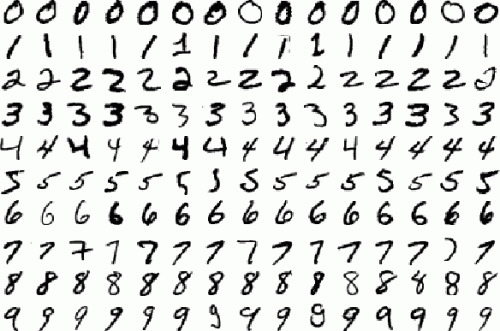
\includegraphics[width=90mm]{./images/mnistdigits.jpg}
\caption{Example MNIST digit images \label{overflow}}
\end{figure}

This example downloads and imports the training and testing datasets from a public Amazon S3 bucket (\url{https://h2o-public-test-data.s3.amazonaws.com/bigdata/laptopt/mnist/train.csv.gz} and same for \texttt{test.csv.gz}).
The training file is 13MB and the testing file is 2.1MB. The data is downloaded directly, so the data import speed is dependent on download speed.  Files can be imported from a variety of sources, including local file systems or shared file systems such as NFS, S3 and HDFS.

\newpage
\waterExampleInR
To run the MNIST example in R, use the following: 
\lstinputlisting[style=R]{DeepLearning_Vignette_code_examples/deeplearning_importfile_example.R}

\waterExampleInPython
To run the MNIST example in Python, use the following: 
\lstinputlisting[style=python]{DeepLearning_Vignette_code_examples/deeplearning_importfile_example.py}

\newpage
\subsection{Performing a Trial Run}
\label{ssec:TrialRun} 

The example below illustrates how the default settings provide the relative simplicity underlying most H2O Deep Learning model parameter configurations. The first $28^2 = 784$ values of each row represent the full image and the final value denotes the digit class. 

Rectified linear activation is popular with image processing and has previously performed well on the MNIST database. Dropout has been known to enhance performance on this dataset as well, so we train our model accordingly. 


To perform the trial run in R, use the following: 

\waterExampleInR
\lstinputlisting[style=R]{DeepLearning_Vignette_code_examples/deeplearning_examplerun.R}

\newpage

To perform the trial run in Python, use the following: 

\waterExampleInPython
\lstinputlisting[style=python]{DeepLearning_Vignette_code_examples/deeplearning_examplerun.py}

\noindent
The model runs for only 10 epochs since it is just meant as a trial run. In this trial run, we also specified the validation set as the test set.  In addition to (or instead of) using a validation set, another option to estimate generalization error is N-fold cross-validation.

\newpage
\subsubsection{N-fold Cross-Validation} 

If the value specified for \texttt{nfolds} is a positive integer, N-fold cross-validation is performed on the \texttt{training\_frame} and the cross-validation metrics are computed and stored as model output.  To disable cross-validation, use \texttt{nfolds=0}, which is the default value.  

To save the predicted values generated during cross-validation, set the\\ \texttt{keep\_cross\_validation\_predictions} parameter to true.  This enables calculation of custom cross-validated performance metrics for the R or Python model.  

Advanced users can also specify a \texttt{fold\_column} that specifies the holdout fold associated with each row. By default, the holdout \texttt{fold\_assignment} is random, but other schemes such as round-robin assignment using the modulo operator are also supported.  

To run the cross-validation example in R, use the following: 

\waterExampleInR
\lstinputlisting[style=R]{DeepLearning_Vignette_code_examples/deeplearning_crossval.R}

\newpage
To run the cross-validation example in Python, use the following: 

\waterExampleInPython
\lstinputlisting[style=python]{DeepLearning_Vignette_code_examples/deeplearning_crossval.py}

\subsubsection{Extracting and Handling the Results} 

We can now extract the parameters of our model, examine the scoring process, and make predictions on new data.  The \texttt{h2o.performance} function in R returns all pre-computed performance metrics for the training/validation set or returns cross-validated metrics for the training set, depending on model configuration. 

An equivalent \texttt{model\_performance} method is available in Python, as well as utility functions that return specific metrics, such as mean square error (MSE) or area under curve (AUC).  Examples shown below use the previously-trained \texttt{model} and \texttt{model\_cv} objects.

\newpage
To view the model results in R, use the following: 

\waterExampleInR
\lstinputlisting[style=R]{DeepLearning_Vignette_code_examples/deeplearning_inspect_model.R}


To view the model results in Python, use the following: 

\waterExampleInPython
\lstinputlisting[style=python]{DeepLearning_Vignette_code_examples/deeplearning_inspect_model.py}


\noindent
The training error value is based on the parameter \texttt{score\_training\_samples}, which specifies the number of randomly sampled training points used for scoring (the default value is 10,000 points). The validation error is based on the parameter \texttt{score\_validation\_samples}, which configures the same value on the validation set (by default, this is the entire validation set).

In general, choosing a greater number of sampled points leads to a better understanding of the model's performance on your dataset; setting either of these parameters to 0 automatically uses the entire corresponding dataset for scoring. However, either method allows you to control the minimum and maximum time spent on scoring with the \texttt{score\_interval} and \texttt{score\_duty\_cycle} parameters.

If the parameter \texttt{overwrite\_with\_best\_model} is enabled, these scoring parameters also affect the final model. This option selects the model that achieved the lowest validation error during training (based on the sampled points used for scoring) as the final model after training. If a dataset is not specified as the validation set, the training data is used by default; in this case, either the \texttt{score\_training\_samples} or \texttt{score\_validation\_samples} parameter will control the error computation during training and consequently, which model is selected as the best model.

Once we have a satisfactory model (as determined by the validation or cross-validation metrics), use the \texttt{h2o.predict()} command to compute and store predictions on new data for additional refinements in the interactive data science process.\nowidow[4]

To view the predictions in R, use the following: 

\waterExampleInR
\lstinputlisting[style=R]{DeepLearning_Vignette_code_examples/deeplearning_predict.R}

\newpage
To view the predictions in Python, use the following: 

\waterExampleInPython
\lstinputlisting[style=python]{DeepLearning_Vignette_code_examples/deeplearning_predict.py}

\subsection{Web Interface} 

H2O R users have access to an intuitive web interface for H2O, Flow, to mirror the model building process in R. After loading data or training a model in R, point your browser to your IP address and port number (e.g., localhost:54321) to launch the web interface. From here, you can click on \textsc{Admin} $>$ \textsc{Jobs} to view specific details about your model. You can also click on \textsc{Data} $>$ \textsc{List All Frames} to view all current H2O frames. 

H2O Python users can connect to Flow the same way as R users: launch an instance of H2O, then launch your browser and enter \texttt{localhost:54321} (or your custom IP address) in the address bar. Python users can also use iPython notebook to run examples. Launch iPython notebook in Terminal using \texttt{ipython notebook}, and a browser window should automatically launch the iPython interface. Otherwise, launch your browser and enter \texttt{localhost:8888} in the address bar. 

\subsubsection{Variable Importances} 

To enable variable importances, setting the \texttt{variable\_importances} to true. This feature allows us to view the absolute and relative predictive strength of each feature in the prediction task.  Each H2O algorithm class has its own methodology for computing variable importance.  

H2O's Deep Learning uses the Gedeon method (\href{http://cs.anu.edu.au/people/Tom.Gedeon/pdfs/ContribDataMinv2.pdf}{Gedeon, 1997}), which is disabled by default since it can be slow for large networks.  If variable importance is a top priority in your analysis, consider training a Distributed Random Forest (DRF) model and comparing the generated variable importances.

The following code demonstrates training using the \texttt{variable\_importances} option and extracting the variable importances from the trained model.  From the web UI, you can also view a visualization of the variable importances.

\waterExampleInR
To generate variable importances in R, use the following: 

\lstinputlisting[style=R]{DeepLearning_Vignette_code_examples/deeplearning_varimp.R}

\waterExampleInPython
To generate variable importances in Python, use the following: 
\lstinputlisting[style=python]{DeepLearning_Vignette_code_examples/deeplearning_varimp.py}

\subsubsection{Java Model} 

To access Java code to use to build the current model in Java, click the \textsc{Preview POJO} button at the
bottom of the model results. This button generates a POJO model that can be used in a Java application independently of H2O. 

To download the model:
\begin{enumerate}
\item Open the terminal window.
\item Create a directory where the model will be saved.
\item Set the new directory as the working directory.
\item Follow the curl and java compile commands displayed in the instructions at the top of the Java model.
\end{enumerate}

For more information on how to use an H2O POJO, refer to the \textbf{POJO Quick Start Guide} at {\url{https://github.com/h2oai/h2o-3/blob/master/h2o-docs/src/product/howto/POJO_QuickStart.md}}. 

\subsection{Grid Search for Model Comparison} 
\label{ssec:GridSearch}

H2O supports model tuning in  grid search by allowing users to specify sets of values for parameter arguments and observe changes in model behavior. An example in R is provided below; the Python grid search API is currently in development.   

In this example, three different network topologies and two different $\ell_1$ norm weights are specified. This grid search model trains six different models using all possible combinations of these parameters; other parameter combinations can be specified for a larger space of models. Note that the models will most likely converge before the default value of \texttt{epochs}, since early stopping is enabled.

Grid search provides more subtle insights into the model tuning and selection process by inspecting and comparing our trained models after the grid search process is complete. To learn how and when to select different parameter configurations in a grid search, refer to {\textbf{\nameref{sec:Parameters}}} for parameter descriptions and configurable values. 


To run a grid search in R, use the following:

\waterExampleInR
\lstinputlisting[style=R]{DeepLearning_Vignette_code_examples/deeplearning_gridsearch.R}



To run a grid search in Python, use the following:

\waterExampleInPython
\lstinputlisting[style=python]{DeepLearning_Vignette_code_examples/deeplearning_gridsearch.py}

\normalsize
\noindent

To view the results of the grid search in R, use the following: 

\waterExampleInR
\lstinputlisting[style=R]{DeepLearning_Vignette_code_examples/deeplearning_gridsearch_result.R}

\medskip

To view the results of the grid search in Python, use the following: 

\waterExampleInPython
\lstinputlisting[style=python]{DeepLearning_Vignette_code_examples/deeplearning_gridsearch_result.py}


\subsection{Checkpoint Models}

To resume model training, use checkpoint model keys (\texttt{model\_id}) to incrementally train a specific model using more iterations, more data, different data, and so forth. To further train the initial model, use it (or its key) as a checkpoint argument for a new model.

To get the best possible model in a general multi-node setup, we recommend building a model with \texttt{train\_samples\_per\_iteration=-2} (default, auto-tuning) and saving it to disk so that you’ll have at least one saved model.

To improve this initial model, start from the previous model and add iterations by building another model, specifying \texttt{checkpoint=previous\_model\_id}, and changing \texttt{train\_samples\_per\_iteration}, \texttt{target\_ratio\_comm\_to\_comp},
or other parameters. Many parameters can be changed between checkpoints, especially those that affect regularization or performance tuning.

Checkpoint restart suggestions:

\begin{enumerate}
\item For multi-node only: Leave \texttt{train\_samples\_per\_iteration=-2}, increase \texttt{target\_ratio\_comm\_to\_comp} from 0.05 to 0.25 or 0.5 (more communication). This should lead to a better model when using multiple nodes. Note: No affect on single-node performance at all, since there is no actual communication needed.
\item For both single and multi-node (bagging-like): Explicitly set \\\texttt{train\_samples\_per\_iteration=N}, where $N$ is the number of training samples for the whole cluster to train with for one iteration. Each of the $n$ nodes will then train on $N/n$ randomly chosen rows for each iteration. Obviously, a good choice for $N$ depends on the dataset size and the model complexity. Refer to the logs to see what values of $N$ are used in option 1 (when auto-tuning is enabled). Typically, option 1 is sufficient.
\item For both single and multi-node: Change regularization parameters such as \texttt{l1}, \texttt{l2}, \texttt{max\_w2}, \texttt{input\_dropout\_ratio}, \texttt{hidden\_dropout\_ratios}. For best results, build the first model with \texttt{RectifierWithDropout} and \texttt{input\_dropout\_ratio=0} and \texttt{hidden\_dropout\_ratios} of all \texttt{0}s, just to be able to enable dropout regularization later. Hidden dropout is often used for initial models, since it often improves generalization. Input dropout is especially useful if there is some noise in the input.
\end{enumerate}

Options 1 and 3 should result in a good model. Of course, grid search can be used with checkpoint restarts to scan a broad range of good continuation models.

In the R example below, \texttt{model\_grid@model\_ids[[1]]} represents the highest-performing model from the grid search used for additional training. For checkpoint restarts, the response column, training, and validation datasets must match.  In addition, the model architecture, such as \texttt{hidden = c(32,32,32)} in the example below, must match.

To restart training in R using a checkpoint model, use the following: 

\waterExampleInR
\lstinputlisting[style=R]{DeepLearning_Vignette_code_examples/deeplearning_checkpoint.R}

The Python example uses the ``trial run'' model  as the checkpoint model.

\waterExampleInPython
\lstinputlisting[style=python]{DeepLearning_Vignette_code_examples/deeplearning_checkpoint.py}

\noindent
Checkpointing can also be used to reload existing models that were saved to disk in a previous session. For example, we can save and reload a model by running the following commands.


To save a model in R, use the following: 

\waterExampleInR
\lstinputlisting[style=R]{DeepLearning_Vignette_code_examples/deeplearning_savemodel.R}


To save a model in Python, use the following: 

\waterExampleInPython
\lstinputlisting[style=python]{DeepLearning_Vignette_code_examples/deeplearning_savemodel.py}

\noindent
After restarting  H2O, load the saved model by specifying the host and saved model file path. \textbf{Note}: The saved model must be reloaded using a compatible H2O version (i.e., the same version used to save the model).

\newpage
To load a saved model in R, use the following: 

\waterExampleInR
\lstinputlisting[style=R]{DeepLearning_Vignette_code_examples/deeplearning_loadmodel_checkpoint.R}

To load a saved model in Python, use the following: 

\waterExampleInPython
\lstinputlisting[style=python]{DeepLearning_Vignette_code_examples/deeplearning_loadmodel_checkpoint.py}


\noindent
You can also use the following commands to retrieve a model from its H2O key. This is useful if you have created an H2O model using the web interface and want to continue the modeling process in R.

To retrieve a model in R using its key, use the following: 

\waterExampleInR
\lstinputlisting[style=R]{DeepLearning_Vignette_code_examples/deeplearning_getmodel.R}

To retrieve a model in Python using its key, use the following: 

\waterExampleInPython
\lstinputlisting[style=python]{DeepLearning_Vignette_code_examples/deeplearning_getmodel.py}

\subsection{Achieving World-Record Performance}

Without distortions, convolutions, or other advanced image processing techniques, the best-ever published test set error for the MNIST dataset is $0.83$\% by Microsoft. After training for $2,000$ epochs (which took about four hours) on four compute nodes, we obtain a test set error of $0.87\%$. 

After training for $8,000$ epochs (which took about ten hours) on ten nodes, we obtain a test set error of $0.83\%$, which is the current world-record, notably achieved using a distributed configuration and with a simple 1-liner from R:

\waterExampleInR
\lstinputlisting[style=R]{DeepLearning_Vignette_code_examples/deeplearning_mnist_record.R}

\subsection{Computational Performance}
There are many parameters that affect the computational performance of H2O Deep Learning, but the default values should result in good performance for most problems. 

An in-depth study of the computational performance characteristics of H2O Deep Learning with complete code examples and results can be found in our blog post, \textbf{Definitive Performance Tuning Guide for Deep Learning}, available at \url{http://h2o.ai/blog/2015/08/deep-learning-performance/}.

The parallel scalability of H2O for the MNIST dataset on 1 to 63 compute nodes is shown in the figure below.
\begin{figure}[h!]
\centering
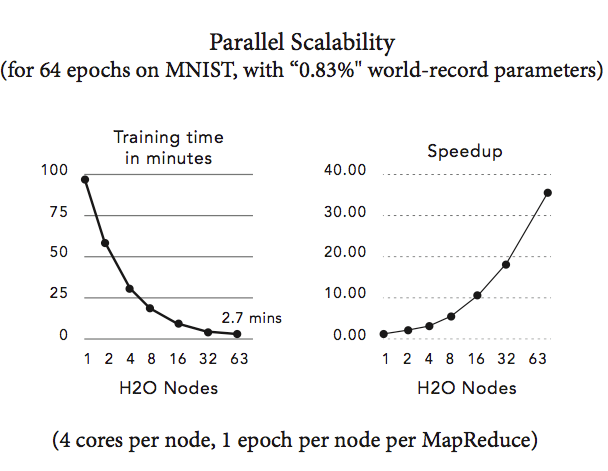
\includegraphics[scale=0.6]{scalability_new.png}
\end{figure}

\newpage
\section{Deep Autoencoders}
\label{sec:DeepAutoencoders}  
This section describes the use of deep autoencoders for Deep Learning. 
\subsection{Nonlinear Dimensionality Reduction} 
Previous sections discussed purely supervised Deep Learning tasks. However, Deep Learning can also be used for unsupervised feature learning or, more specifically, nonlinear dimensionality reduction  (\href{http://www.cs.toronto.edu/~hinton/science.pdf}{Hinton et al, 2006}). 

Based on the diagram of a three-layer neural network with one hidden layer below, if our input data is treated as labeled with the same input values, then the network is forced to learn the identity via a nonlinear, reduced representation of the original data. 

\begin{figure}[h!]
\centering
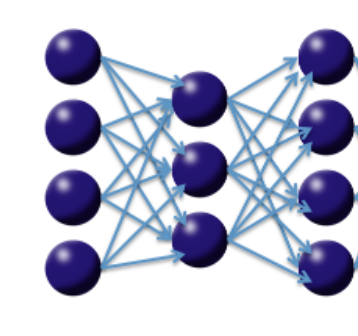
\includegraphics[scale=0.5]{autoencoder.png}
\end{figure}

This type of algorithm, called a deep autoencoder, has been used extensively for unsupervised, layer-wise pre-training of supervised Deep Learning tasks. Here we discuss the autoencoder's ability to discover anomalies in data. 



\subsection{Use Case: Anomaly Detection} %%TODO: do we still want to use this example?
For the deep autoencoder model described above, if enough training data resembling some underlying pattern is provided, the network will train itself to easily learn the identity when confronted with that pattern. However, if an anomalous test point does not match the learned pattern, the autoencoder will likely have a high error rate in reconstructing this data, indicating anomalous data.

This framework is used to develop an anomaly detection demonstration using a deep autoencoder. The dataset is an ECG time series of heartbeats and the goal is to determine which heartbeats are outliers. The training data (20 ``good" heartbeats) and the test data (training data with 3 ``bad" heartbeats appended for simplicity) can be downloaded directly into the H2O cluster, as shown below.  Each row represents a single heartbeat. 

%\begin{lstlisting}[style=R]
%train_ecg.hex = h2o.uploadFile(h2o_server, path="ecg_train.csv", header=F, sep=",", key="train_ecg.hex") 
%test_ecg.hex = h2o.uploadFile(h2o_server, path="ecg_test.csv", header=F, sep=",", key="test_ecg.hex") 
%
%#Train deep autoencoder learning model on "normal" training data, y ignored 
%anomaly_model = h2o.deeplearning(x=1:210, y=1, train_ecg.hex, activation = "Tanh", classification=F, autoencoder=T, hidden = c(50,20,50), l1=1E-4, 
%epochs=100)                 
%                              
%#Compute reconstruction error with the Anomaly detection app (MSE between output layer and input layer)
%recon_error.hex = h2o.anomaly(test_ecg.hex, anomaly_model)
%                              
%#Pull reconstruction error data into R and plot to find outliers (last 3 heartbeats)
%recon_error = as.data.frame(recon_error.hex)
%recon_error
%plot.ts(recon_error)
%
%#Note: Testing = Reconstructing the test dataset
%test_recon.hex = h2o.predict(anomaly_model, test_ecg.hex) 
%head(test_recon.hex)              
%
%\end{lstlisting}

\newpage
\waterExampleInR
\lstinputlisting[style=R]{DeepLearning_Vignette_code_examples/deeplearning_anomaly.R}

\newpage

To run the anomaly detection example in Python, use the following:
 
\waterExampleInPython
\lstinputlisting[style=python]{DeepLearning_Vignette_code_examples/deeplearning_anomaly.py}

\newpage
\subsubsection{Stacked Autoencoder}
It can be difficult to obtain convergence for deep autoencoders, especially since H2O attempts to train all layers at once without imposing symmetry conditions on the network topology (arbitrary configuration of layers is allowed). To train a deep autoencoder layer by layer, follow the \texttt{R} code example here:

\url{https://github.com/h2oai/h2o-3/blob/master/h2o-r/tests/testdir_algos/deeplearning/runit_deeplearning_stacked_autoencoder_large.R}.


\section{Parameters}
\label{sec:Parameters}

Logical indicates the parameter requires a value of either \texttt{TRUE} or \texttt{FALSE}. 

\begin{itemize}

\item \texttt{x}: Specifies the vector containing the names of the predictors in the model. No default.

\item \texttt{y}: Specifies the name of the response variable in the model. No default.

\item \texttt{training\_frame}: Specifies an \texttt{H2OFrame} object containing the variables in the model.  No default.

\item \texttt{model\_id}: (Optional) Specifies the unique ID associated with the model. If a value is not specified, an ID is generated automatically. 

\item \texttt{overwrite\_with\_best\_model}: Logical. If enabled, overwrites the final model with the best model scored during training. The default is true.

\item \texttt{validation\_frame}: (Optional) Specifies an \texttt{H2OFrame} object representing the validation dataset used for the confusion matrix. If a value is not specified and \texttt{nfolds = 0}, the training data is used by default. 

\item \texttt{checkpoint}: (Optional) Specifies the model checkpoint (either an \\ \texttt{H2ODeepLearningModel} or a key) from which to resume training. 

\item \texttt{autoencoder}: Logical. Enables autoencoder. The default is false. Refer to the {\textbf{\nameref{sec:DeepAutoencoders}}} section for more details.

\item \texttt{use\_all\_factor\_levels}: Logical. Uses all factor levels of categorical variance. Otherwise, omits the first factor level without loss of accuracy. Useful for variable importances and auto-enabled for autoencoder.  The default is true. Refer to the {\textbf{\nameref{sec:DeepAutoencoders}}} section for more details.

\item \texttt{activation}: Specifies the nonlinear, differentiable activation function used in the network. The options are \texttt{Tanh, TanhWithDropout, Rectifier, RectifierWithDropout, Maxout,} or \\\texttt{MaxoutWithDropout}. The default is \texttt{Rectifier}. Refer to the {\textbf{\nameref{sssec:ActivationLoss}}} and {\textbf{\nameref{ssec:Regularization}}} sections for more details.

\item \texttt{hidden}: Specifies the number and size of each hidden layer in the model. For example, if \texttt{c(100,200,100)} is specified, a model with 3 hidden layers is generated. The middle hidden layer will have 200 neurons and the first and third hidden layers will have 100 neurons each. The default is \texttt{c(200,200)}. For grid search, use the following format: \texttt{list(c(10,10), c(20,20))}. Refer to the section on  {\textbf{\nameref{ssec:TrialRun}}} for more details. 

\item \texttt{epochs}: Specifies the number of iterations or passes over the training dataset (can be fractional). For initial grid searches, we recommend starting with lower values. The value allows continuation of selected models and can be modified during checkpoint restarts. The default is 10.

\item \texttt{train\_samples\_per\_iteration}: Specifies the number of training samples (globally) per MapReduce iteration. The following special values are also supported: 
\begin{itemize}
\item \texttt{0} (one epoch)
\item \texttt{-1} (all available data including replicated training data);
\item \texttt{-2} (auto-tuning; default)
\end{itemize}
Refer to {\textbf{\nameref{sssec:TrainSamplesPerIter}}} for more details.

\item \texttt{seed}: Specifies the random seed controls sampling and initialization. Reproducible results are only expected with single-threaded operations (i.e. running on one node, turning off load balancing, and providing a small dataset that fits in one chunk).  In general, the multi-threaded asynchronous updates to the model parameters will result in intentional race conditions and non-reproducible results.  The default is a randomly generated number.

\item \texttt{adaptive\_rate}: Logical.  Enables adaptive learning rate (ADADELTA). The default is true. Refer to {\textbf{\nameref{sssec:AdaptiveLearning}}} for more details.

\item \texttt{rho}: Specifies the adaptive learning rate time decay factor. This parameter is similar to momentum and relates to the memory for prior weight updates. Typical values are between 0.9 and 0.999. The default value is 0.99. %The value of \texttt{rho} must be greater than zero if \texttt{epsilon} is greater than zero. 
Refer to {\textbf{\nameref{sssec:AdaptiveLearning}}} for more details. 

\item \texttt{epsilon}: When enabled, specifies the second of two hyperparameters for the adaptive learning rate. This parameter is similar to learning rate annealing during initial training and momentum at later stages where it assists progress. Typical values are between 1e-10 and 1e-4. This parameter is only active if \texttt{adaptive\_rate} is enabled. The default is 1e-8. %The value of \texttt{epsilon} must be greater than zero if \texttt{rho} is greater than zero.   
Refer to {\textbf{\nameref{sssec:AdaptiveLearning}}} for more details.

\item \texttt{rate}: Specifies the learning rate, $\alpha$. Higher values lead to less stable models, while lower values result in slower convergence. The default is 0.005.  %%is this still supported? 

\item \texttt{rate\_annealing}: Reduces the learning rate to ``freeze'' into local minima in the optimization landscape. The annealing learning rate is calculated as \texttt{(rate)} / (1 + \texttt{rate\_annealing} * $N$), where $N$ is the number of training samples.  It is the inverse of the number of training samples required to cut the learning rate in half.  If adaptive learning is disabled, the default value is 1e-6. Refer to {\textbf{\nameref{sssec:RateAnnealing}}} for more details.

\item \texttt{rate\_decay}:  Controls the change of learning rate across layers. The learning rate decay factor between layers is calculated as ($L$-th layer: \texttt{rate} * \texttt{rate\_decay\^} ($L$-1)). If adaptive learning is disabled, the default is 1.0. 

\item \texttt{momentum\_start}: Controls the amount of momentum at the beginning of training when adaptive learning is disabled. The default is 0. Refer to {\textbf{\nameref{sssec:MomentumTraining}}} for more details.

\item \texttt{momentum\_ramp}: If the value for \texttt{momentum\_stable} is greater than\\ \texttt{momentum\_start}, increases momentum for the duration of the learning.  The ramp is measured in the number of training samples and can be enabled when adaptive learning is disabled. The default is 1 million (1e6). Refer to {\textbf{\nameref{sssec:MomentumTraining}}} for more details.

\item \texttt{momentum\_stable}: Specifies the final momentum value after the number of training samples specified for \texttt{momentum\_ramp} when adaptive learning is disabled. The training momentum is applied for any additional training. The default is 0.  Refer to {\textbf{\nameref{sssec:MomentumTraining}}} for more details.

\item \texttt{nesterov\_accelerated\_gradient}:  Logical.  Enables the Nesterov accelerated gradient descent method, which is a modification to the traditional gradient descent for convex functions. The method relies on gradient information at various points to build a polynomial approximation that minimizes the residuals in fewer iterations of the descent. This parameter is only active if the adaptive learning rate is disabled.  When adaptive learning is disabled, the default is true. Refer to {\textbf{\nameref{sssec:MomentumTraining}}} for more details.

\item \texttt{input\_dropout\_ratio}: Specifies the fraction of the features for each training row to omit from training to improve generalization. The default is 0, which always uses all features.  Refer to {\textbf{\nameref{ssec:Regularization}}} for more details.

\item \texttt{hidden\_dropout\_ratios}:  Specifies the fraction of the inputs for each hidden layer to omit from training to improve generalization. The default is 0.5 for each hidden layer.  Refer to {\textbf{\nameref{ssec:Regularization}}} for more details.

\item \texttt{l1}: Specifies the $\ell_1$ (L1) regularization, which constrains the absolute value of the weights (can add stability and improve generalization, causes many weights to become 0). The default is 0, for no L1 regularization. Refer to {\textbf{\nameref{ssec:Regularization}}} for more details.

\item \texttt{l2}: L2 regularization, which constrains the sum of the squared weights and can add stability and improve generalization by reducing many weights). The default is 0, which disables L2 regularization. Refer to {\textbf{\nameref{ssec:Regularization}}} for more details.

\item \texttt{max\_w2}: Specifies the maximum for the sum of the squared incoming weights for a neuron. This tuning parameter is especially useful for unbound activation functions such as Maxout or Rectifier. The default, which is positive infinity, leaves this maximum unbounded.

\item \texttt{initial\_weight\_distribution}: Specifies the distribution from which to draw the initial weights. Select \texttt{Uniform, UniformAdaptive} or \texttt{Normal}. The default is \texttt{UniformAdaptive}. Refer to {\textbf{\nameref{sssec:Initialization}}} for more details.

\item \texttt{initial\_weight\_scale}: Specifies the scale of the distribution function for uniform or normal distributions. For uniform distributions, the values are drawn uniformly from \texttt{initial\_weight\_scale, \\ initial\_weight\_scale}. For normal distributions, the values are drawn from a normal distribution with a standard deviation of \\ \texttt{initial\_weight\_scale}. The default is 1. Refer to {\textbf{\nameref{sssec:Initialization}}} for more details.

\item \texttt{loss}: Specifies the loss option: \texttt{Automatic, CrossEntropy} (classification only), \texttt{Quadratic, Absolute}, or \texttt{Huber}. The default is \texttt{Automatic}. Refer to {\textbf{\nameref{sssec:ActivationLoss}}} for more details.

\item \texttt{distribution}: Specifies the distribution function of the response: \texttt{AUTO, bernoulli, multinomial, poisson, gamma, \\ tweedie, laplace, huber,} or \texttt{gaussian}. 

\item \texttt{tweedie\_power}: Specifies the Tweedie power when \texttt{distribution} is  \texttt{tweedie}. The range is from 1.0 to 2.0. 

\item \texttt{score\_interval}: Specifies the minimum time (in seconds) between model scoring. The actual interval is determined by the number of training samples per iteration and the scoring duty cycle. To use all training set samples, specify \texttt{0}. The default is 5.

\item \texttt{score\_training\_samples}: Specifies the number of training samples to randomly sample for scoring. To select the entire training dataset, specify \texttt{0}.  The default is 10000.

\item \texttt{score\_validation\_samples}: Specifies the number of validation dataset points for scoring. Can be randomly sampled or stratified if  \texttt{balance\_classes} is enabled and \texttt{score\_validation\_sampling} is \texttt{Stratified}. To select the entire validation dataset, specify \texttt{0}, which is the default.

\item \texttt{score\_duty\_cycle}: Specifies the maximum duty cycle fraction for model scoring on both training and validation samples and diagnostics such as computation of feature importances. Lower values result in more training, while higher values produce more scoring. The default is 0.1.

\item \texttt{classification\_stop}: Specifies the stopping criterion for classification error (1 - accuracy) on the training data scoring dataset.  When the error is at or below this threshold, training stops.  The default is 0.  To disable, specify \texttt{-1}. 

\item \texttt{regression\_stop}: Specifies the stopping criterion for regression error (MSE) on the training data scoring dataset. When the error is at or below this threshold, training stops. The default is 1e-6.  To disable, specify \texttt{-1}.

\item \texttt{stopping\_rounds}: Early stopping based on convergence of \\\texttt{stopping\_metric}. Stop if simple moving average of length k of the \texttt{stopping\_metric} does not improve for k:=\texttt{stopping\_rounds} scoring events. Can only trigger after at least 2k scoring events. To disable, specify \texttt{0}.

\item \texttt{stopping\_metric}: Metric to use for early stopping (\texttt{AUTO}: \texttt{logloss} for classification, \texttt{deviance} for regression). Can be any of \texttt{AUTO, deviance, logloss, MSE, AUC, r2, misclassification}.

\item \texttt{stopping\_tolerance}: Relative tolerance for metric-based stopping criterion Relative tolerance for metric-based stopping criterion (stop if relative improvement is not at least this much).

\item \texttt{quiet\_mode}: Logical. Enables quiet mode for less output to standard output. The default is false.

\item \texttt{max\_confusion\_matrix\_size}: For classification models, specifies the maximum size (in terms of classes) for displaying the confusion matrix. This option helps avoid printing extremely large confusion matrices. The default is 20.

\item \texttt{max\_hit\_ratio\_k}: For multi-class only. Specifies the maximum number (top $K$) of predictions to use for hit ratio computation. To disable, specify \texttt{0}. The default is 10.

\item \texttt{balance\_classes}: Logical. For imbalanced data, the training data class counts can be artificially balanced by over-sampling the minority classes and under-sampling the majority classes so that each class  contains the same number of observations.  This can result in improved predictive accuracy.  Over-sampling  uses replacement, rather than simulating new observations. The \texttt{max\_after\_balance\_size} parameter specifies the total number of observations after balancing. The default is false.
%This means that the maximum number of obs will be 5*N, where N is the number of observations in the original (unbalanced) training set.  If you want the balanced training set to have the same number of obs as the original training set, then set this to argument to 1.  

\item \texttt{class\_sampling\_factors}: Specifies the desired over/under-sampling ratios per class (in lexicographic order). Only applies to classification when \texttt{balance\_classes} is enabled. If not specified, the ratios are automatically computed to obtain class balancing during training.

\item \texttt{max\_after\_balance\_size}: When classes are balanced, limits the resulting dataset size to the specified multiple of the original dataset size. This is the maximum relative size of the training data after balancing class counts and can be less than 1.0. The default is 5.

\item \texttt{score\_validation\_sampling}: Specifies the method used to sample the validation dataset for scoring. The options are \texttt{Uniform} and \texttt{Stratified}. The default is \texttt{Uniform}.

%\item \texttt{diagnostics}: (Deprecated) Logical. Gather diagnostics for hidden layers, such as mean and root mean squared (RMS) values of learning rate, momentum, weights and biases. Since deprecation, diagnostics are always enabled (set to true).

\item \texttt{variable\_importances}: Logical. Computes variable importances for input features using the Gedeon method. Uses the weights connecting the input features to the first two hidden layers. The default is false, since this can be slow for large networks. 

\item \texttt{fast\_mode}: Logical. Enables fast mode, a minor approximation in back-propagation that should not significantly affect results. The default is true.

\item \texttt{ignore\_const\_cols}: Logical. Ignores constant training columns, since no information can be gained anyway.  The default is true.

\item \texttt{force\_load\_balance}:  Logical. Forces extra load balancing to increase training speed for small datasets to keep all cores busy. The default is true.

\item \texttt{replicate\_training\_data}:  Logical. Replicates the entire training dataset on every node for faster training on small datasets. The default is true.

\item \texttt{single\_node\_mode}:  Logical. Runs Deep Learning on a single node for fine-tuning model parameters. Can be useful for faster convergence during checkpoint restarts after training on a very large number of nodes (for fast initial convergence). The default is false.

\item \texttt{shuffle\_training\_data}: Logical. Shuffles training data on each node. This option is recommended if training data is replicated on $N$ nodes and the number of training samples per iteration is close to $N$ times the dataset size, where all nodes train with almost all of the data. It is automatically enabled if the number of training samples per iteration is set to -1 (or to $N$ times the dataset size or larger).  The default is false.

\item \texttt{sparse}: Logical. Enables sparse data handling (more efficient for data with lots of 0 values).
The default is false.

\item \texttt{col\_major}: (Deprecated) Logical. Uses a column major weight matrix for the input layer; can speed up forward propagation, but may slow down backpropagation. The default is false.

\item \texttt{average\_activation}: Specifies the average activation for the sparse autoencoder (Experimental).
The default is 0.

\item \texttt{sparsity\_beta}: Specify the sparsity-based regularization optimization (Experimental).  The default is 0. 

\item \texttt{max\_categorical\_features}:  Specifies the maximum number of categorical features in a column, enforced via hashing (Experimental).  The default is $2^{31}-1$ (\texttt{Integer.MAX\_VALUE} in Java).

\item \texttt{reproducible}: Logical. Forces reproducibility on small data; slow, since it only uses one thread.  The default is false.

\item \texttt{export\_weights\_and\_biases}: Logical. Exports the neural network weights and biases as an \texttt{H2OFrame}.  The default is false.

% TO DO: Should these be added?  They are in the Java code, but not documented elsewhere
%  public boolean _elastic_averaging = false;
%  public double _elastic_averaging_moving_rate = 0.9;
%  public double _elastic_averaging_regularization = 1e-3;
%
%  // stochastic gradient descent: mini-batch size = 1
%  // batch gradient descent: mini-batch size = # training rows
%  public int _mini_batch_size = 1;

\item \texttt{offset\_column}:  Specifies the offset column by column name.  Regression only.  Offsets are per-row ``bias values'' that are used during model training. For Gaussian distributions, they can be seen as simple corrections to the response (y) column. Instead of learning to predict the response value directly, the model learns to predict the (row) offset of the response column. For other distributions, the offset corrections are applied in the linearized space before applying the inverse link function to get the actual response values. 

\item \texttt{weights\_column}: Specifies the weights column by column name, which must be included in the specified \texttt{training\_frame}. \textit{Python only}: To use a weights column when passing an H2OFrame to \texttt{x} instead of a list of column names, the specified \texttt{training\_frame} must contain the specified \texttt{weights\_column}. Weights are per-row observation weights. This is typically the number of times a row is repeated, but non-integer values are supported as well. During training, rows with higher weights matter more, due to the larger loss function pre-factor.

\item \texttt{nfolds}: (Optional) Specifies the number of folds for cross-validation. % If the number of folds is greater than or equal to 2, then validation must remain empty. 
The default is 0, which disables cross-validation.

\item \texttt{fold\_column}: (Optional) Specifies the name of the column with the cross-validation fold index assignment per observation; the folds are supplied by the user. 

\item \texttt{fold\_assignment}: Specifies the cross-validation fold assignment scheme if \texttt{nfolds} is greater than zero and \texttt{fold\_column} is not specified. The options are \texttt{AUTO, Random,} or \texttt{Modulo}. 

\item \texttt{keep\_cross\_validation\_predictions}: Logical.  Specify whether to keep the predictions of the cross-validation models.  The default is false.

\end{itemize}

% TO DO:  Replicate this in other booklets (or move the generic part to ./common)
\section{Common R Commands}
\begin{itemize}

\item \texttt{library(h2o)}: Imports the H2O R package.

\item \texttt{h2o.init()}:  Connects to (or starts) an H2O cluster.

\item \texttt{h2o.shutdown()}: Shuts down the H2O cluster.

\item \texttt{h2o.importFile(path)}: Imports a file into H2O.

\item \texttt{h2o.deeplearning(x,y,training\_frame,hidden,epochs)}:\\ Creates a Deep Learning model.

\item \texttt{h2o.grid(algorithm,grid\_id,...,hyper\_params = list())}: Starts H2O grid support and gives results.

\item \texttt{h2o.predict(model, newdata)}: Generate predictions from an H2O model on a test set.

\end{itemize}

% TO DO:  Replicate this in other booklets (or move the generic part to ./common)
\section{Common Python Commands}
\begin{itemize}
%TO DO: Anisha
\item \texttt{import h2o}:  Imports the H2O Python package.

\item \texttt{h2o.init()}:  Connects to (or starts) an H2O cluster.

\item \texttt{h2o.shutdown()}: Shuts down the H2O cluster.

\item \texttt{h2o.import\_file(path)}: Imports a file into H2O.

\item \texttt{model = H2ODeepLearningEstimator(hidden, epochs)}: \\ Creates a Deep Learning model.

\item \texttt{model.train(x, y, training\_frame)}: \\ Trains our Deep Learning model.

%\item \texttt{h2o.grid} (not yet available): Starts H2O grid support and gives results.

\item \texttt{h2o.predict(model, newdata)}: Generate predictions from an H2O model on a test set.

\end{itemize}

\newpage

\section{References}

\bibliographystyle{plainnat}  

\nobibliography{bibliography.bib} %hides entire bibliography so just \bibentry items are included - use \bibentry{bibname} (where bibname is the entry name in the bibliography) to include entries from bibliography.bib; double brackets {{ are required in .bib file to preserve capitalization

\bibentry{DLcode}

\bibentry{dlarch}

\bibentry{backprop}

\bibentry{maxout}

\bibentry{hogwild}

\bibentry{featuredetectors}

\bibentry{momentum}

\bibentry{adadelta}

\bibentry{mnist}

\bibentry{neuralnet}

\bibentry{performance}

\bibentry{h2osite}

\bibentry{h2odocs}

\bibentry{h2ogithubrepo}

\bibentry{h2odatasets}

\bibentry{h2ojira}

\bibentry{stream}

\bibentry{rdocs}




%%\textbf{H2O Training}:    {\url{http://learn.h2o.ai/}}

%%\textbf{H2O Training Scripts and Data}: {\url{http://data.h2o.ai/}} 

%\textbf{H2O YouTube Channel}: 

%{\url{https://www.youtube.com/user/0xdata}}


%\textbf{Data mining of inputs: Analysing magnitude and functional measures}. {Gedeon, 2012}.  \\
 %\href{http://cs.anu.edu.au/people/Tom.Gedeon/pdfs/ContribDataMinv2.pdf}{http://cs.anu.edu.au/people/Tom.Gedeon/pdfs/ContribDataMinv2.pdf}

%%TODO: add Arno's performance guide blog post after it is updated; need a good way to include bar charts for results - can re-create in Photoshop if needed, but we should definitely include a link to the script

%%TODO: Remove `maxout` refs, add "mini-badge" parameter?

\newpage
\section{Authors}

\textbf{Arno Candel}

Arno is the Chief Architect of H2O, a distributed and scalable open-source machine learning platform. He is also the main author of H2O Deep Learning.  Arno holds a PhD and Masters summa cum laude in Physics from ETH Zurich, Switzerland. He has authored dozens of scientific papers and is a sought-after conference speaker. Arno was named “2014 Big Data All-Star” by Fortune Magazine. Follow him on Twitter: @ArnoCandel.

\textbf{Erin LeDell}

Erin is a Statistician and Machine Learning Scientist at H2O.ai. She is the main author of H2O Ensemble. 
Erin received her Ph.D. in Biostatistics with a Designated Emphasis in Computational Science and Engineering from University of California, Berkeley. Her research focuses on ensemble machine learning, learning from imbalanced binary-outcome data, influence curve based variance estimation and statistical computing. She also holds a B.S. and M.A. in Mathematics.

\textbf{Viraj Parmar}

Viraj is studying applied mathematics at Princeton. Prior to joining H2O.ai as a former data and math hacker intern, Viraj worked in a research group at the MIT Center for Technology and Design. His interests are in software engineering and large-scale machine learning. Apart from work, Viraj enjoys reading, sampling new cuisines, and traveling with his family.

\textbf{Anisha Arora}

Anisha is a software intern who is a senior at Cupertino High School. She enjoys programming and is interested in machine learning. She likes to swim, play the piano and violin, and tutor in science and math subjects at her school.


\textbf{Jessica Lanford}

Jessica is a word hacker and seasoned technical communicator at H2O.ai. She brings our product to life by documenting the many features and functionality of H2O. Having worked for some of the top companies in technology including Dell, AT$\&$T, and Lam Research, she is an expert at translating complex ideas to digestible articles.

\end{document}
